\documentclass[11pt]{article}

\usepackage[margin=1.1in]{geometry}
\usepackage{graphicx}
\usepackage{booktabs}
\usepackage{amsmath,amssymb}
\usepackage{microtype}
\usepackage{xcolor}
\usepackage[font=small,labelfont=bf]{caption}
\usepackage{enumitem}
\usepackage{multirow}
\usepackage[round]{natbib}
\usepackage{float}
\usepackage[colorlinks=true,linkcolor=blue!50!black,citecolor=blue!50!black,urlcolor=blue!50!black]{hyperref}

\graphicspath{{../figures/}{../figures/whitepaper/}}

% ---- shorthand ----
\newcommand{\fprother}{\ensuremath{\mathrm{FPR}_{\mathrm{other}}}}
\newcommand{\tprat}[1]{\ensuremath{\mathrm{TPR}@#1\%}}
\newcommand{\ms}[2]{\ensuremath{#1{\scriptstyle\,\pm #2}}}
\newcommand{\vbest}{v14b}

\title{\bfseries Catching Cross-Generator Email Impersonation with\\ Content-Invariant Authorship Embeddings}
\author{Armaan Patankar\\ \small KL Convergence \quad \texttt{armaan@klconvergence.com}}
\date{July 2026}

\begin{document}
\maketitle

\begin{abstract}
\noindent
Business email compromise increasingly relies on large language models (LLMs) to imitate a specific
person's writing style. We describe a sender-verification system that enrolls each sender's style as a
centroid in an authorship embedding space and flags messages whose style does not match the claimed
sender. The central technical difficulty is \emph{cross-generator generalization}: a detector trained
against forgeries from one LLM learns generator-specific artifacts and collapses on forgeries from
unseen models (\tprat{1} $0.91 \to 0.045$). We show that the two obvious drop-in fixes both fail on
this threat --- zero-shot machine-generated-text detectors score at or below chance
(AUC 0.49--0.54) on few-shot \emph{imitation} emails, and an off-the-shelf content-independent style
embedding underperforms our fine-tuned encoder on every axis. The fix that works is retraining the
authorship backbone itself, with two levers: (i) synthetic hard negatives from \emph{multiple}
generator vendors, evaluated only on \emph{held-out} vendors, and (ii) identity diversity, expanding
training authors from 44 to 844. A completed $2{\times}2$ factorial shows the levers are
\emph{super-additive}: identity diversity alone does nothing for forgery detection, but it amplifies
the synthetic-negative gain from $+0.23$ to $+0.37$ AUC. The final model reaches
AUC \ms{0.980}{0.003} on forgeries from generators never seen in training (91\% caught at a 5\%
false-alarm budget), holds a wrong-human false-accept guardrail at 8\%, transfers to novel vendors
outside both training and evaluation (AUC 0.996), and improves cross-topic authorship verification
(PAN $0.779 \to 0.857$). All results are reported as mean$\pm$std over evaluation seeds, with a
training-seed reproduction.
\end{abstract}

\tableofcontents

%=====================================================================
\section{Introduction}
\label{sec:intro}

Impersonation is the core mechanic of business email compromise (BEC): a message arrives that
claims to be from a colleague or executive, and its content and address look legitimate. Modern
LLMs sharply lower the cost of the strongest form of this attack --- given a handful of a victim's
real emails, an LLM can produce fluent text \emph{in that person's approximate style}, defeating
both content-based filters and human suspicion.

Our system defends at the layer the attacker must ultimately forge: \textbf{authorship}. Every
sender in an organization is enrolled by encoding their verified historical emails into a style
embedding space and storing a per-sender profile (centroid, spread, and count). An incoming message
claiming to be from that sender is encoded and scored by its distance to the profile; large
deviations are flagged. The encoder is trained once, on public corpora --- it never sees the deployment
organization's senders at training time and is never retrained at deployment; new senders are
enrolled with forward passes only.

This paper documents the system and, more importantly, the empirical path to making it work against
LLM forgeries. Three findings organize the paper:

\begin{enumerate}[leftmargin=2em]
\item \textbf{The central problem is cross-generator generalization
      (\S\ref{sec:gap}).} Training against forgeries from a single LLM produces a detector of
      \emph{that LLM's artifacts}, not of forgery: on forgeries from unseen generators, the catch
      rate at 1\% false-alarm collapsed from 0.91 to 0.045. Consequently, every headline number in
      this paper is computed on forgeries from generators \emph{excluded from training}
      (Claude~3.5~Haiku and Gemini~2.5~Flash), and we additionally spot-check vendors outside both
      training and evaluation.
\item \textbf{Drop-in alternatives fail on imitation (\S\ref{sec:pivots}).} Zero-shot
      machine-generated-text (MGT) detectors (Fast-DetectGPT, Binoculars) score at or below chance
      on few-shot imitation emails --- text prompted to mimic a specific human is precisely the case
      the MGT literature warns about. An off-the-shelf content-independent style embedding
      (StyleDistance) is worse than our fine-tuned encoder on every evaluation slice. The fix has
      to be trained into our own authorship backbone.
\item \textbf{Two levers close the gap, and they interact super-additively
      (\S\ref{sec:method}--\ref{sec:ablations}).} Multi-vendor synthetic hard negatives are the
      primary lever ($+0.23$ AUC); expanding training identities from 44 to 844 authors does
      nothing \emph{by itself} for forgery detection but amplifies the synthetic lever to $+0.37$,
      yielding held-out AUC \ms{0.980}{0.003}. Identity diversity's standalone payoff is
      content-invariance --- a separate axis on which it improves cross-topic verification from
      0.779 to 0.857--0.879.
\end{enumerate}

We also report what did not work and what remains open: a scorer that Goodharts its
threshold when synthetics become easy (\S\ref{sec:guardrail}), a length-invariance weakness that
survives every version (\S\ref{sec:limits}), and the evaluation practices --- held-out generators,
a wrong-human guardrail metric, multi-seed error bars, a training-seed reproduction ---
that we believe are the minimum for trusting results in this adversarial setting.

%=====================================================================
\section{Threat model and task}
\label{sec:threat}

\paragraph{Setting.} A deployment organization provides a historical archive of verified-genuine
email. The system runs in two phases. \emph{Enrollment}: each sender's emails are preprocessed
(reply chains and signatures stripped; URLs, addresses, and phone numbers masked), encoded, and
summarized into a profile $\{\mu_s, \sigma_s, k_s\}$ --- centroid, mean cosine spread, and email
count. \emph{Scoring}: an incoming email claiming sender $s$ is encoded and scored against
$\{\mu_s, \sigma_s, k_s\}$, returning a score in $[0,1]$ and a verdict (genuine / suspicious /
abstain when $k_s < 5$).

\paragraph{Adversaries.} Two impostor classes claim sender $s$'s identity:
\begin{itemize}[leftmargin=2em]
\item \textbf{Wrong-human impostors}: mail genuinely written by a different person. This is the
      classical authorship-verification negative and is comparatively easy for our encoder
      (AUC ${\approx}0.97$ across all versions).
\item \textbf{LLM forgeries}: text produced by an LLM \emph{prompted with several of $s$'s real
      emails} as style exemplars (few-shot imitation). This models an attacker who has compromised
      or scraped samples of the victim's writing --- the realistic BEC case --- and is the hard class.
\end{itemize}
We assume the attacker can use any current or future LLM vendor, so the defender cannot count
on having trained against the attacker's generator. We do not assume the attacker has query access
to the deployed detector (adaptive attacks are out of scope; see \S\ref{sec:limits}).

\paragraph{Operating requirements.} The deployment metric is the catch rate at a small false-alarm
budget, \tprat{5} (secondarily \tprat{1}), on forgeries from \emph{held-out} generators, subject to
a \textbf{guardrail}: at the chosen threshold, the false-accept rate on wrong-human impostors,
\fprother{}, must stay ${\leq}0.10$. A system that catches forgeries by flagging everything
unusual --- including legitimate mail from a colleague --- is not deployable.

%=====================================================================
\section{Related work}
\label{sec:related}

\paragraph{Authorship representation.} LUAR \citep{riverasoto2021} learns universal authorship
representations by contrasting episodes (bags of texts) by the same author, pretrained at Reddit
scale; it is the backbone we fine-tune. Content-independent style embeddings
\citep{wegmann2022,styledistance2024} attack the confound that same-author text pairs also share
topic; StyleDistance trains on synthetic paraphrase pairs that hold content fixed while varying
style. Cross-topic authorship verification is the standard stress test \citep{kestemont2020}.

\paragraph{Machine-generated-text detection.} Zero-shot detectors score text by likelihood
statistics under reference models --- Fast-DetectGPT's conditional probability curvature
\citep{fastdetectgpt2023} and Binoculars' cross-perplexity ratio \citep{binoculars2024}.
Benchmarks consistently find that \emph{trained} MGT detectors fail to transfer across generators
\citep{raid2024}, and that adversarial or stylized generations defeat zero-shot detectors. Our
results sharpen this for the impersonation threat: few-shot imitations of a specific human are
\emph{more} human-like than real email under these detectors' statistics (\S\ref{sec:pivots}).

\paragraph{Positioning.} Our approach is personalized authorship verification used as a forgery
detector: rather than asking ``was this text machine-generated?'' (generator-dependent, brittle),
we ask ``was this text written by the person it claims to be from?'' --- a question whose signal
belongs to the \emph{sender}, not to the attacker's generator. The project's arc is evidence that
this is the durable formulation.

%=====================================================================
\section{System}
\label{sec:system}

\subsection{Encoder}
The backbone is LUAR-MUD \citep{riverasoto2021} with episode pooling: $K$ emails from one sender
form an episode and produce one L2-normalized style embedding (projection dim 128, max length 512
tokens). We fine-tune with LoRA \citep{hu2022} ($r{=}16$, $\alpha{=}32$, dropout 0.05) on the
query/key/value projections; the backbone stays frozen. Training batches are built by a $P{\times}K$
sampler ($P$ senders $\times$ $K{=}8$ emails, batch size 128) with random crop augmentation
(30\% of texts cropped to 5--60 words) to reduce length sensitivity.

\paragraph{Why an authorship backbone.} In an early bake-off, topic-pretrained encoders
(RoBERTa, MPNet) trained with the same contrastive recipe reached validation AUROC ${\approx}0.53$
--- near chance --- while LUAR-MUD reached 0.956. Masked-LM embeddings cluster by topic, and no
amount of LoRA fine-tuning on 44 senders fixed the inductive bias; authorship pretraining is
load-bearing. (A diagnostic: RoBERTa's same-sender similarity was high, but so was its
different-sender similarity --- nothing discriminative was learned.)

\subsection{Objective}
The loss is an episodic supervised-contrastive objective: within each batch, embeddings sharing a
sender label attract and all others repel, with temperature $\tau{=}0.05$
\citep{khosla2020}. Episodes are formed with variable support size (2--6 emails), and a plain
SupCon term is mixed in with weight 0.5. Lower temperature weights the hardest negatives most ---
which, by construction (below), are LLM imitations of the anchor sender.

\subsection{Synthetic hard negatives}
\label{sec:synthetics}
For each training sender we generate \emph{imitation} emails: an external LLM is prompted with
several of the sender's real emails and asked to write new mail as that person. Each imitation set
is registered as its own identity, \texttt{alice\_\_syn}, distinct from \texttt{alice}. A
\texttt{SyntheticBalancedSampler} guarantees $n_{\mathrm{syn}}{=}4$ (real, synthetic) sender pairs
per batch, so every batch forces the loss to separate real-Alice from LLM-Alice --- the model must
find stylistic features the LLM failed to reproduce.

Two rules were learned the hard way and are enforced in code:
\begin{itemize}[leftmargin=2em]
\item \textbf{LLM text is never a positive.} An earlier version used LLM-generated cross-register
      text as additional positives for the sender; it regressed wrong-human verification and was
      banned (confirmed by a five-arm ablation isolating the objective change).
\item \textbf{Checkpoint selection must not watch synthetics alone.} A synthetic-only model monitor
      selects checkpoints that leak up to 60\% of wrong-human mail. The training monitor is
      $\min(\text{pAUC}_{\mathrm{other}}, \text{pAUC}_{\mathrm{synthetic}})$ at 5\% FPR, the
      worst case of the two impostor axes.
\end{itemize}

\subsection{Scoring}
\label{sec:scoring}
At inference, the query embedding $q$ is compared to the claimed sender's profile. Two scorers
matter in this paper:
\begin{itemize}[leftmargin=2em]
\item \texttt{linear\_z3} (baseline): $z = (1-\cos(q,\mu_s))/\sigma_s$, score
      $=\max(0, 1-z/3)$. Simple, no per-sender fitting beyond spread.
\item \texttt{mahalanobis} (deployed): per-sender Mahalanobis distance under a Ledoit--Wolf
      shrunk covariance \citep{ledoitwolf2004} fit to the enrollment embeddings, gated by
      enrollment count: senders with $k<5$ fall back to cosine ranking (a covariance cannot be
      estimated), and $k<5$ also triggers the abstain tier.
\end{itemize}
Both scorers \emph{rank} wrong-human impostors nearly identically (AUC 0.94--0.97); they differ in
where a synthetic-anchored threshold lands, which decides the guardrail
(\S\ref{sec:guardrail}).

%=====================================================================
\section{Evaluation protocol}
\label{sec:protocol}

\paragraph{The held-out-generator rule.} Forgeries used in training come from
\textbf{GPT-4o-mini} and \textbf{Llama-3.1-70B} (plus DeepSeek in one version). Forgeries used for
\emph{all headline evaluations} come from \textbf{Claude-3.5-Haiku} and \textbf{Gemini-2.5-Flash},
which are never used in training, for any version. A further spot-check uses
\textbf{Qwen-2.5-72B} and \textbf{DeepSeek-V3} --- outside both the training \emph{and} evaluation
sets (\S\ref{sec:novelvendor}). Every version of the system is graded on the same held-out pool.

\paragraph{Probe.} The evaluation pool profiles 44 Enron senders (the post-filter maximum) with
$k{=}8$ enrollment emails each, and scores 264 genuine queries, 327 held-out LLM forgeries
(172 Claude, 155 Gemini), and 600 wrong-human queries. Metrics: AUC (forgery vs.\ genuine),
\tprat{5} and \tprat{1} at synthetic-anchored thresholds, \fprother{} at the 5\% threshold
(the guardrail), and AUC on genuine-vs-wrong-human ranking. Each metric carries a 1000-sample
paired bootstrap; in addition, the entire probe (sender, enrollment, query, and impostor draws) is
repeated over \textbf{5 seeds} and reported as mean$\pm$std throughout.

\paragraph{The in-distribution trap.} Per-run validation panels (negatives drawn from that run's
\emph{own} training generators) are useful for watching convergence and useless for comparison:
the single-generator model posts validation \tprat{1} $= 0.74$ while catching 4.5\% of held-out
forgeries. All numbers in this paper come from the fixed held-out probe above, never from training
dashboards.

\paragraph{Secondary axes.} Content-invariance is measured on PAN~2020 cross-topic authorship
verification pairs \citep{kestemont2020} (clean out-of-domain: never trained on) and a held-out
150-author slice of the Blog Authorship Corpus \citep{schler2006}; length and register robustness
on stratified Enron pair slices.

%=====================================================================
\section{The central problem: cross-generator generalization}
\label{sec:gap}

\subsection{Single-generator training learns the generator, not forgery}
\label{sec:v11collapse}
The v11 model --- the strongest single-generator configuration, trained with Mistral-7B-family
imitations --- looked excellent in distribution: \tprat{1} $= 0.91$ against Mistral forgeries. On
the held-out Claude+Gemini pool the same model collapses to \tprat{1} $= 0.045$ and AUC $0.75$
(multi-seed: AUC \ms{0.690}{0.020}). The learned ``LLM-ness'' feature was a Mistral artifact
detector. This single number reframed the project: the metric that matters is
\textbf{TPR at low FPR on held-out generators}, and everything after v11 is an attempt to move it.

\subsection{Failed alternative 1: zero-shot MGT detectors}
\label{sec:pivots}
If forgery detection cannot be trained per-generator, generator-agnostic zero-shot detectors are
the natural drop-in. We evaluated two, at their recommended settings, on exactly our held-out pool
(genuine = real Enron mail, forgeries = few-shot imitations by Claude/Gemini):

\begin{table}[h]
\centering
\small
\begin{tabular}{lccccc}
\toprule
Detector & Claude & Gemini & Pooled & Len-matched & \tprat{1} \\
\midrule
Fast-DetectGPT & \textbf{0.399} & 0.693 & 0.538 & 0.536 & 0.012 \\
Binoculars & \textbf{0.398} & 0.582 & 0.485 & 0.523 & 0.016 \\
\emph{Authorship signal (v12, ref.)} & \emph{0.829} & \emph{0.746} & \emph{0.854} & --- & \emph{0.13} \\
\bottomrule
\end{tabular}
\caption{Zero-shot MGT detectors on few-shot imitation emails (held-out pool); all columns except
\tprat{1} are AUC. Both put Claude imitations \emph{below chance}: the imitations are more
``human-like'' under likelihood statistics than real, messy corporate email. Length-matching does
not rescue them.}
\label{tab:zeroshot}
\end{table}

This is not a weak-detector artifact --- two unrelated methods agree, after length control. Few-shot
imitation produces fluent, low-perplexity text \emph{by construction}; ``is this generic LLM
text?'' is the wrong question for this threat. It also reinterprets what v11--v13's trained
detector head was doing: not detecting LLM-ness, but generator artifacts --- explaining both its
in-distribution strength and its held-out collapse.

\subsection{Failed alternative 2: off-the-shelf style embeddings}
If the issue is content sensitivity, a content-independent style embedding trained elsewhere might
substitute for ours. StyleDistance \citep{styledistance2024}, evaluated over the same
out-of-domain pair files as our encoder, is worse on every slice --- including the cross-topic slice
its training specifically targets:

\begin{table}[h]
\centering
\small
\begin{tabular}{lccc}
\toprule
Slice (pairwise AUC) & StyleDistance & Fine-tuned LUAR (v12) & $\Delta$ \\
\midrule
PAN cross-topic & 0.748 & 0.779 & $-0.031$ \\
Blog & 0.793 & 0.839 & $-0.046$ \\
Mixed-length pairs & 0.580 & 0.931 & $-0.351$ \\
Claude / Gemini forgery & 0.560 / 0.583 & 0.829 / 0.746 & $-0.27$ / $-0.16$ \\
\bottomrule
\end{tabular}
\caption{An off-the-shelf content-independent embedding does not transfer to email. The lesson is
not that content-independence is wrong --- it is that it must be trained into \emph{our} encoder,
not imported.}
\label{tab:styledistance}
\end{table}

Together, \S\ref{sec:pivots} narrows the design space to one path: \textbf{retrain the authorship
backbone itself} to be generator-robust and content-invariant. These two negative results were
obtained \emph{before} committing GPU budget to that path, and they are why the rest of the paper
is about training levers rather than architecture swaps.

%=====================================================================
\section{Method: two levers}
\label{sec:method}

Each version changes one thing; all are graded on the identical held-out probe
(Table~\ref{tab:main}).

\paragraph{v12 --- generator diversity.} Train the synthetic hard negatives with \emph{two} vendors
(GPT-4o-mini + Llama-3.1-70B), holding out Claude+Gemini. Hypothesis: diversity in the training
adversary transfers to unseen adversaries. Result: AUC $0.690 \to 0.871$; per-generator
Claude $0.639 \to 0.829$, Gemini $0.614 \to 0.746$. Confirmed --- the first real fix.

\paragraph{v13 --- more generator diversity (plateau).} Add DeepSeek as a third vendor with more
per-sender volume. Result: \ms{0.872}{0.021} --- statistically flat versus v12. Generator count had
stopped paying; the bottleneck was elsewhere. The diagnosis: with only 44 training identities, the
model's notion of ``this person's style'' is too coarse to distinguish a good imitation from the
real author, regardless of how many generators supply imitations.

\paragraph{v14 --- identity diversity (a clean split of effects).} Expand training identities from
44 Enron senders to \textbf{844 authors} by adding 800 authors from the Blog Authorship Corpus,
forcing the contrastive objective across far more authors and topics. This run dropped synthetics
(a sampler limitation, fixed in \vbest{}). Result: one breakthrough and one collapse.
Content-invariance moved for the first time in the project --- PAN cross-topic
$0.779 \to 0.879$ --- while forgery detection collapsed to \ms{0.610}{0.016} (Claude
$0.829 \to 0.541$), proving synthetics are load-bearing for forgery-catching. As an accidental
ablation, v14 cleanly separates the levers: \emph{identity diversity buys content-invariance;
synthetics buy forgery detection}.

\paragraph{\vbest{} --- the synthesis.} The blocker was the sampler: the old epoch length was set
by the 44 synthetic pairs (${\sim}11$ batches), starving the 800 blog authors. The fixed
synthetic-balanced sampler scales the epoch to the real-author pool (${\sim}105$ batches)
while still guaranteeing synthetic pairs in every batch (verified byte-identical on all
prior configs, which have no unpaired authors). \vbest{} = 844 authors + GPT/Llama synthetics +
the worst-case-anchored monitor. Result: \textbf{AUC \ms{0.980}{0.003}}, better than every
predecessor on every axis simultaneously (Table~\ref{tab:main}, Figure~\ref{fig:progression});
per-generator Claude 0.972, Gemini 0.953.

\begin{figure}[t]
\centering
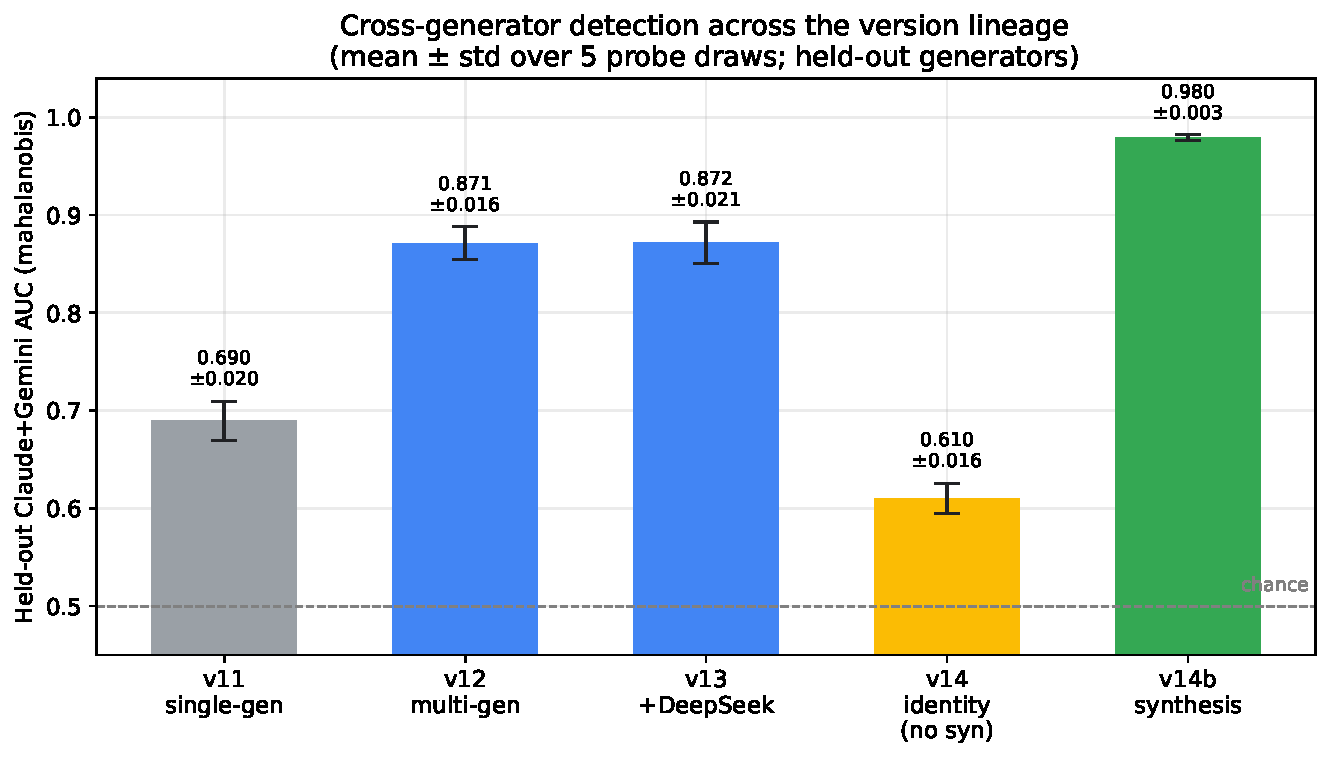
\includegraphics[width=0.9\linewidth]{wp_fig1_multiseed_progression.pdf}
\caption{Held-out Claude+Gemini forgery AUC (Mahalanobis scorer), mean$\pm$std over 5 probe seeds.
Every version-to-version gap is far larger than its seed variance.}
\label{fig:progression}
\end{figure}

%=====================================================================
\section{Main results}
\label{sec:results}

\begin{table}[t]
\centering
\small
\setlength{\tabcolsep}{4.5pt}
\begin{tabular}{llccccc}
\toprule
Version & Change & AUC & \tprat{5} & \tprat{1} & \fprother{}@5 & AUC g/other \\
\midrule
v11 & single generator & \ms{0.690}{0.020} & \ms{0.121}{0.017} & \ms{0.043}{0.012} & \ms{0.000}{0.000} & \ms{0.967}{0.003} \\
v12 & multi-generator & \ms{0.871}{0.016} & \ms{0.453}{0.064} & \ms{0.155}{0.036} & \ms{0.001}{0.001} & \ms{0.965}{0.002} \\
v13 & +3rd vendor & \ms{0.872}{0.021} & \ms{0.499}{0.069} & \ms{0.255}{0.047} & \ms{0.001}{0.001} & \ms{0.970}{0.004} \\
v14 & 844 authors, $-$syn & \ms{0.610}{0.016} & \ms{0.137}{0.015} & \ms{0.060}{0.013} & \ms{0.010}{0.003} & \ms{0.667}{0.015} \\
\textbf{\vbest{}} & \textbf{844 authors, $+$syn} & \textbf{\ms{0.980}{0.003}} & \textbf{\ms{0.909}{0.017}} & \textbf{\ms{0.533}{0.055}} & \textbf{\ms{0.079}{0.014}} & \textbf{\ms{0.967}{0.003}} \\
\bottomrule
\end{tabular}
\caption{Main result: held-out Claude+Gemini pool, Mahalanobis scorer, mean$\pm$std over 5 probe
seeds. AUC is forgery vs.\ genuine; \fprother{}@5 is the wrong-human false-accept rate at the 5\%
operating point (guardrail $\leq 0.10$); AUC g/other is genuine vs.\ wrong-human ranking.}
\label{tab:main}
\end{table}

\subsection{At the operating point}
At the same 5\% false-alarm threshold on the held-out pool (seed-0 probe), v12 and \vbest{} allow
the same genuine mail (251/264) --- but v12 misses 61\% of forgeries (198/327) while \vbest{} misses
12\% (40/327), and both keep wrong-human catch rates high (598 vs.\ 550 of 600). The change a
deployment sees is a $39\% \to 88\%$ forgery catch rate at unchanged false-alarm cost, against
generators the model has never trained on (Figure~\ref{fig:confusion}).

\begin{figure}[t]
\centering
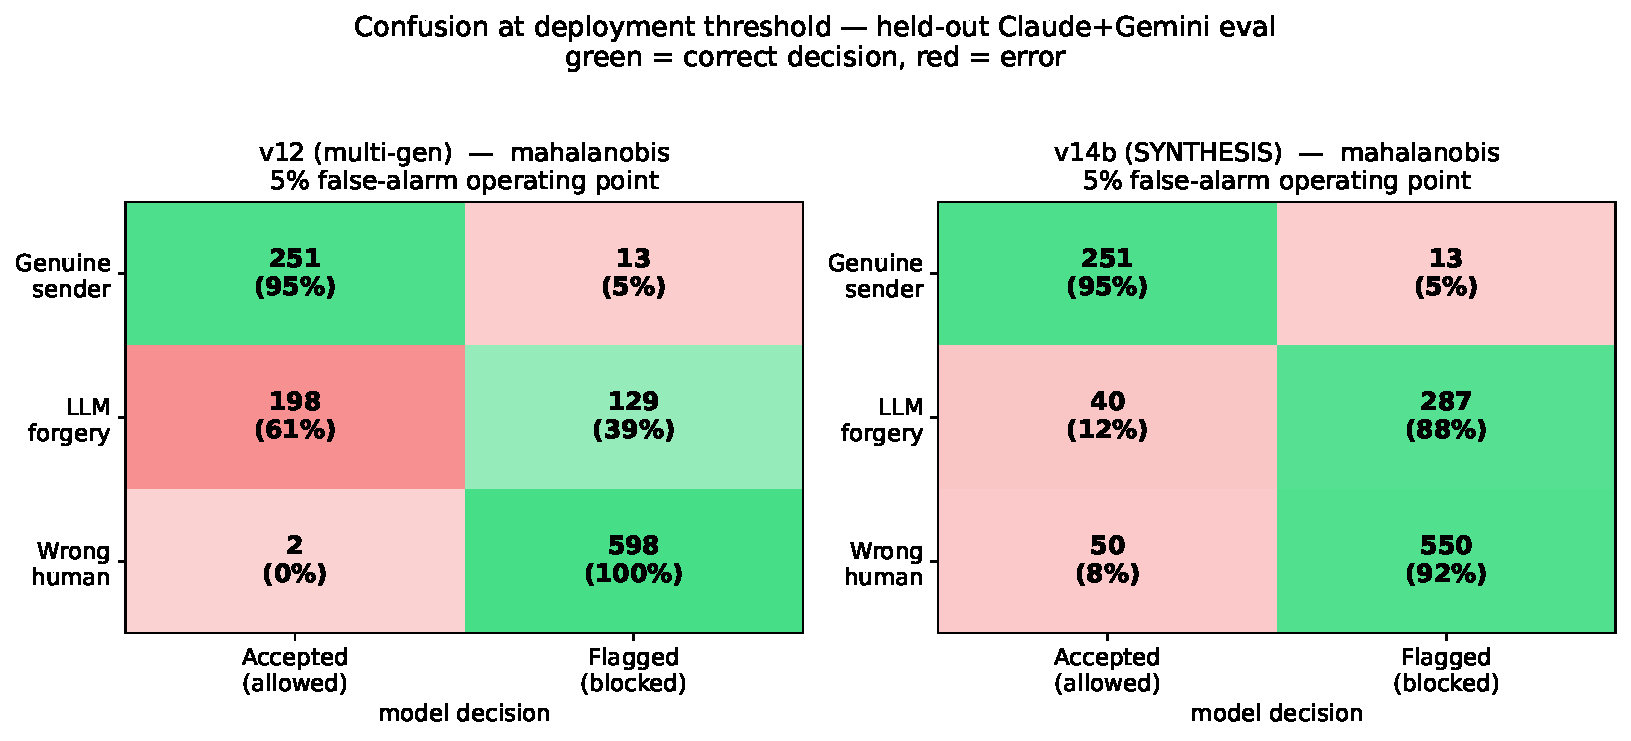
\includegraphics[width=0.95\linewidth]{fig4_confusion_v12_vs_v14b.pdf}
\caption{Confusion at the 5\% false-alarm operating point, held-out pool (probe seed 0): v12 (left)
vs.\ \vbest{} (right).}
\label{fig:confusion}
\end{figure}

\subsection{The guardrail: scorer choice decides deployability}
\label{sec:guardrail}
\vbest{} separates synthetics so well that a threshold anchored on the synthetic pool alone can
land badly for the \emph{wrong-human} axis. Across all 5 seeds:

\begin{table}[h]
\centering
\small
\begin{tabular}{lcc}
\toprule
Scorer & \tprat{5} (forgeries) & \fprother{}@5 (wrong-human leak) \\
\midrule
\texttt{linear\_z3} & \ms{0.943}{0.013} & \ms{0.253}{0.032} \quad breaches guardrail \\
\texttt{mahalanobis} (deployed) & \ms{0.909}{0.017} & \ms{0.079}{0.014} \quad holds $\leq 0.10$ \\
\bottomrule
\end{tabular}
\caption{Scorer choice at the synthetic-anchored 5\% threshold, mean$\pm$std over 5 seeds. Both
scorers \emph{rank} wrong-humans well (AUC 0.94--0.97); the linear scorer simply sits at a bad
threshold. This is an operating-point property, invisible to AUC.}
\label{tab:guardrail}
\end{table}

The deployment rule that follows --- and that the novel-vendor result (\S\ref{sec:novelvendor})
makes even more pointed --- is: \textbf{ship the Mahalanobis scorer and anchor the threshold on the
worst case of the wrong-human and synthetic axes, never on the synthetic pool alone.} The better
the model gets on synthetics, the more degenerate a synthetic-only threshold becomes.

\begin{figure}[t]
\centering
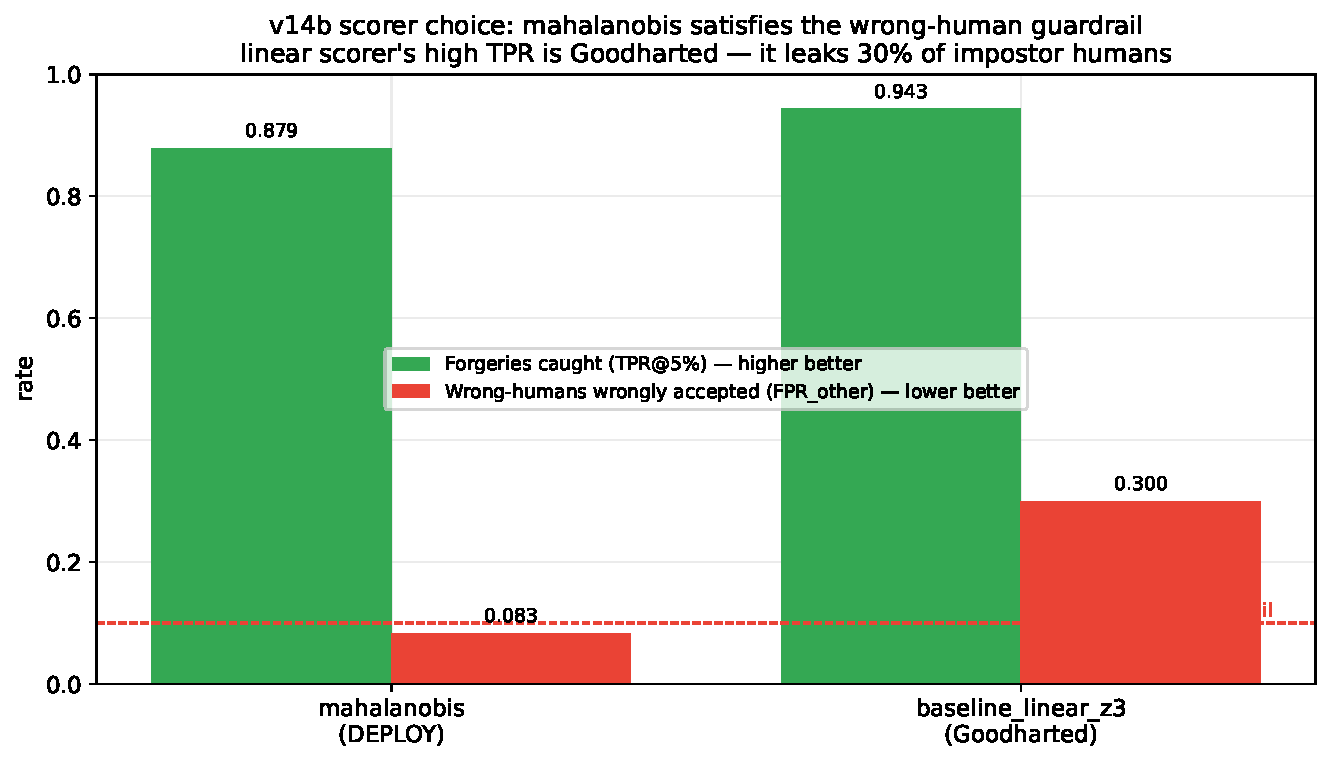
\includegraphics[width=0.85\linewidth]{fig5_guardrail_scorer_choice.pdf}
\caption{Scorer choice at the deployment operating point (seed-0 probe; Table~\ref{tab:guardrail}
gives the multi-seed bands). The linear scorer catches slightly more forgeries but leaks 30\% of
wrong-human impostors; Mahalanobis holds the guardrail.}
\label{fig:guardrail}
\end{figure}

%=====================================================================
\section{Ablations and robustness}
\label{sec:ablations}

\subsection{Identity $\times$ synthetics: a super-additive interaction}
\label{sec:2x2}
The lineage confounds the two levers (v12 changed generators; v14 changed identities \emph{and}
dropped synthetics). We completed the factorial by training the missing corner --- 44 authors
without synthetics, at a step budget between v12's and v14's to avoid an undertraining confound:

\begin{table}[h]
\centering
\small
\begin{tabular}{lcc}
\toprule
Held-out AUC & no synthetics & $+$ synthetics \\
\midrule
44 authors (Enron) & \ms{0.640}{0.012} & \ms{0.871}{0.016} \; (v12) \\
844 authors (Enron+Blog) & \ms{0.610}{0.016} \; (v14) & \textbf{\ms{0.980}{0.003}} \; (\vbest{}) \\
\bottomrule
\end{tabular}
\caption{Identity $\times$ synthetic $2{\times}2$ (held-out Claude+Gemini, Mahalanobis, 5-seed
mean$\pm$std).}
\label{tab:2x2}
\end{table}

Three readings, none visible from the lineage alone:
\begin{itemize}[leftmargin=2em]
\item \textbf{Identity diversity alone does nothing for forgery detection}: $0.640 \to 0.610$
      going $44 \to 844$ authors without synthetics --- flat to slightly negative.
\item \textbf{Synthetics are the primary lever}: $+0.231$ AUC at 44 authors.
\item \textbf{Identity amplifies synthetics}: the synthetic gain grows to $+0.370$ at 844 authors.
      Equivalently, identity expansion only pays off in the presence of synthetics
      ($0.871 \to 0.980$).
\end{itemize}
The precise claim is therefore not ``two independent levers'' but: \emph{identity diversity's
value for catching LLM imitations is unlocked by synthetic hard negatives}. A sharper authorship
space is only useful against forgeries if training also supplies examples of what a forgery is;
conversely, hard negatives are only fully exploitable when the style space is fine-grained enough
to place imitations away from a well-modeled centroid. Identity diversity's \emph{standalone}
payoff is content-invariance (\S\ref{sec:content}), an orthogonal axis. The production model needs
both levers because it faces both failure modes.

\begin{figure}[t]
\centering
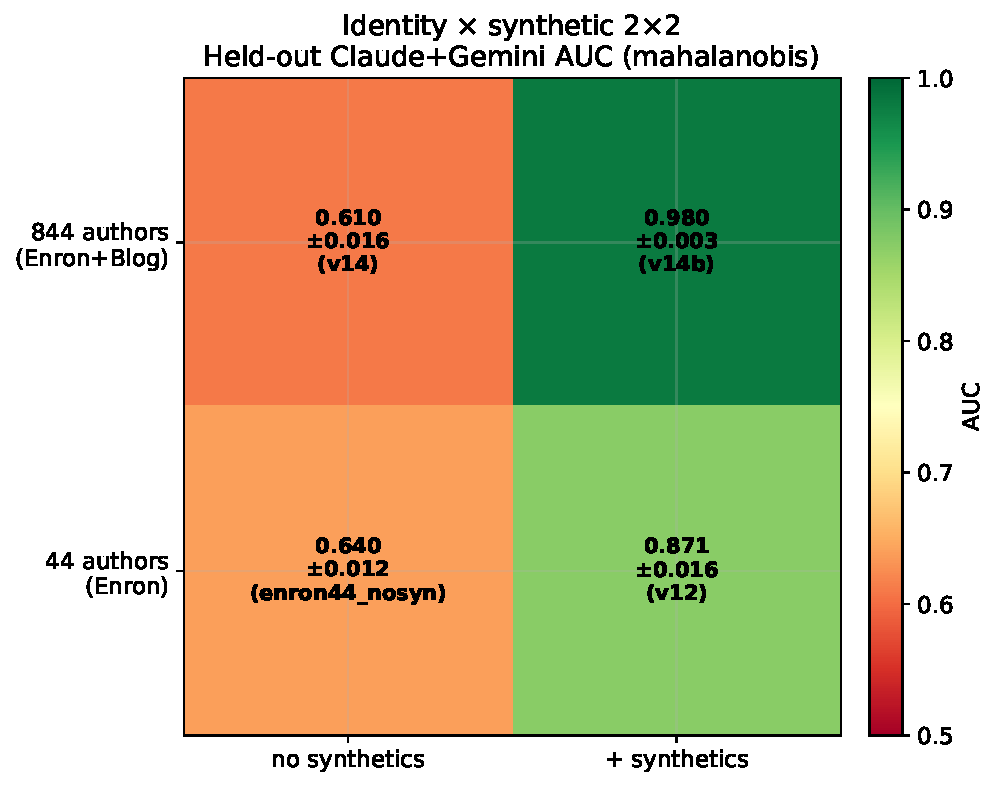
\includegraphics[width=0.8\linewidth]{wp_fig2_2x2_grid.pdf}
\caption{The completed $2{\times}2$. The interaction is super-additive: the whole
(\ms{0.980}{0.003}) exceeds the sum of the parts.}
\label{fig:2x2}
\end{figure}

\subsection{Training-seed reproduction}
\label{sec:seedrepro}
The headline could be a lucky initialization. Retraining \vbest{} from scratch with a different
seed (new weight init and data order) reproduces the ranking within probe noise:
AUC \ms{0.976}{0.005} vs.\ \ms{0.980}{0.003}, guardrail held for both
(\fprother{} \ms{0.038}{0.017} vs.\ \ms{0.079}{0.014}). One honest nuance: the operating-point
tail carries more training-seed variance than AUC --- \tprat{5} moves from \ms{0.909}{0.017} to
\ms{0.867}{0.037} across the two trainings. We therefore report \tprat{5} as a band
(${\sim}0.87$--$0.91$) rather than a point, and recommend per-deployment threshold calibration.

\subsection{Novel-vendor spot-check}
\label{sec:novelvendor}
Held-out Claude+Gemini could in principle have been ``overfit'' through repeated evaluation
across the project. We generated 343 fresh forgeries with \textbf{Qwen-2.5-72B} and
\textbf{DeepSeek-V3} --- vendors outside both the training set and the recurring evaluation set ---
and evaluated blind:

\begin{table}[h]
\centering
\small
\begin{tabular}{lccc}
\toprule
Version & AUC (forgery/genuine) & \tprat{5} & AUC g/other \\
\midrule
v12 & \ms{0.922}{0.005} & \ms{0.630}{0.030} & \ms{0.964}{0.000} \\
\vbest{} & \textbf{\ms{0.996}{0.001}} & \textbf{\ms{0.986}{0.008}} & \ms{0.966}{0.003} \\
\bottomrule
\end{tabular}
\caption{Novel vendors (Qwen-2.5-72B + DeepSeek-V3), never in training or prior evaluation.
Mahalanobis, mean$\pm$std over 3 probe seeds.}
\label{tab:novelvendor}
\end{table}

\vbest{}'s separation is, if anything, \emph{stronger} on the novel vendors --- it did not overfit
to Claude/Gemini. One caveat we report deliberately: on this pool the raw \fprother{}@5 reads
$0.58\pm0.21$. This is a threshold-placement artifact, not a real leak --- with synthetics
near-perfectly separated (AUC 0.996), the 5\%-synthetic-anchored threshold lands in a degenerate
flat region of the score distribution (the $\pm 0.21$ variance is the tell), while wrong-human
\emph{ranking} remains clean (AUC 0.97). This is the strongest demonstration in the paper of the
\S\ref{sec:guardrail} rule: as synthetic separation approaches saturation, a synthetic-anchored
operating point becomes meaningless, and the threshold must be anchored on the wrong-human axis.

\begin{figure}[t]
\centering
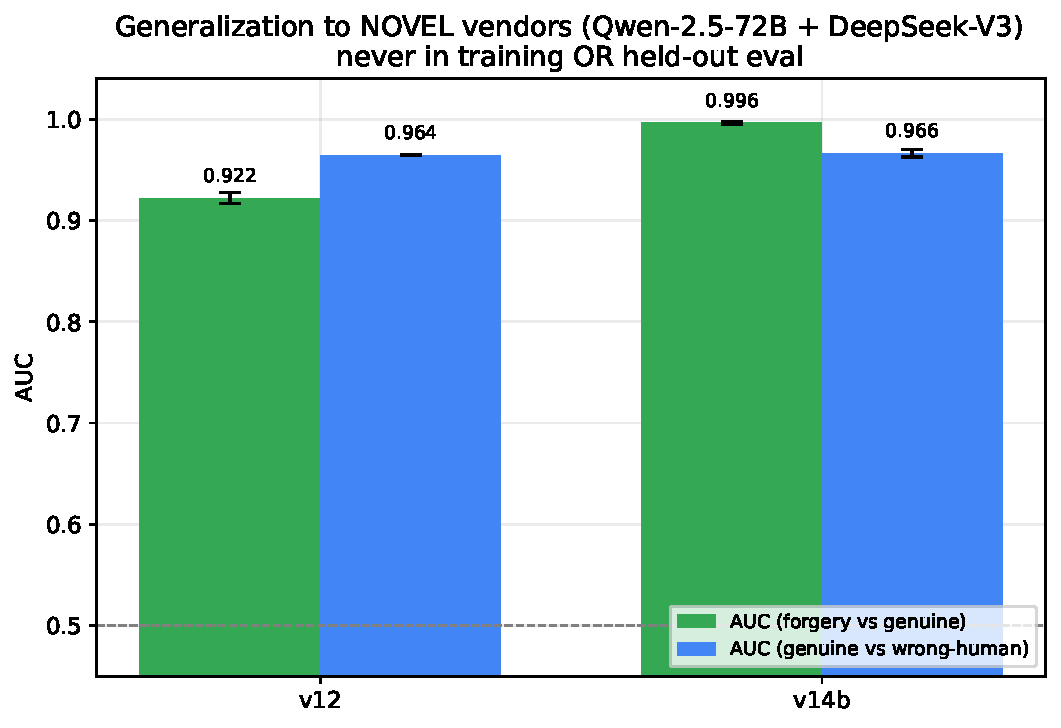
\includegraphics[width=0.85\linewidth]{wp_fig3_novelvendor.pdf}
\caption{Novel-vendor spot-check (Qwen-2.5-72B + DeepSeek-V3): forgery separation (left) and
genuine-vs-wrong-human ranking (right), v12 vs.\ \vbest{}.}
\label{fig:novelvendor}
\end{figure}

\subsection{Content-invariance}
\label{sec:content}
Identity diversity's independent payoff. On PAN cross-topic verification (clean out-of-domain ---
never in training for any version): v12/v13-recipe 0.779 $\to$ v14 0.879 $\to$ \vbest{} 0.857.
On the held-out 150-author blog probe: v12 0.786 $\to$ \vbest{} 0.909 (corroborating, though blog
is partly in-domain for v14/\vbest{} since other blog authors are in training). \vbest{} gives
back a small part of v14's PAN gain (0.879 $\to$ 0.857) in exchange for the forgery axis --- an
acceptable trade, and both far exceed the 0.779 plateau that held from v11 through v13.

%=====================================================================
\section{Limitations}
\label{sec:limits}

\begin{itemize}[leftmargin=2em]
\item \textbf{Sender ceiling.} The cross-generator probe has 44 profiled senders (the post-filter
      maximum of the Enron corpus). AUC and \tprat{5} are tight, but \tprat{1} retains wide
      intervals (${\pm}0.05$--$0.06$ even at the 5-seed mean); enlarging beyond 44 requires a second
      enrollment corpus. Lead with AUC and \tprat{5}.
\item \textbf{Length invariance is the weakest axis.} Verifying a short text against a long one
      remains the worst slice in every version. On enrollment-free pairwise probes over unseen
      senders (v11-era), mixed-length verification was near chance (0.53--0.64); on the current
      enrolled probe \vbest{} reaches AUC 0.930 on mixed-length pairs but only \tprat{5} 0.71 ---
      its weakest slice. The scoring-side mitigation we tested (length-matched enrollment) was
      cleanly refuted (it \emph{discards} length-invariant signal; pAUC@5\% $-0.08$). The open
      levers are length-conditioned thresholds and cross-length hard negatives in training.
\item \textbf{Operating-point tail variance.} \tprat{5} varies ${\sim}{\pm}0.04$ across training
      seeds (\S\ref{sec:seedrepro}); quote it as a band and calibrate thresholds per deployment.
\item \textbf{Blog is partly in-domain.} The clean content-invariance evidence is PAN cross-topic
      (0.857); the blog number (0.909) corroborates but shares a corpus with training.
\item \textbf{Adaptive attackers.} We evaluate few-shot imitation, not an attacker who iterates
      against the deployed detector's scores. Style-space evasion under query access is untested.
\item \textbf{Corpus and language scope.} Training and evaluation are English corporate email and
      blogs; transfer to other languages and registers is unmeasured.
\end{itemize}

%=====================================================================
\section{Deployment recommendations}
\label{sec:deploy}

\begin{enumerate}[leftmargin=2em]
\item \textbf{Ship} the \vbest{} checkpoint with the \textbf{Mahalanobis} scorer
      (cosine fallback and abstain below $k{=}5$ enrollment emails).
\item \textbf{Anchor the operating point on $\min$(wrong-human, synthetic)} --- never on the
      synthetic pool alone (\S\ref{sec:guardrail}, \S\ref{sec:novelvendor}). Expected operating
      behavior at the 5\% budget: forgery catch rate $0.87$--$0.91$, wrong-human false-accept
      ${\leq}0.10$.
\item \textbf{Calibrate per deployment.} The tail is threshold-sensitive; fit the operating point
      on the deployment's own genuine/impostor score distributions. Per-sender or conformal
      calibration is the natural next step.
\item \textbf{Monitor for novel generators.} The novel-vendor result (AUC 0.996) is encouraging,
      but new vendors should be spot-checked as they appear --- generation of a fresh imitation pool
      for a new vendor is an hours-scale, eval-only exercise in this codebase.
\item \textbf{Never retrain on deployment data silently.} The encoder is enrollment-only at
      deployment by design; profile updates are $O(1)$ per email and auditable.
\end{enumerate}

%=====================================================================
\section{Conclusion}
\label{sec:conclusion}

The project's thesis, earned the long way: \textbf{better authorship modeling is what catches LLM
imitations}. Detectors of machine-generated text --- trained or zero-shot --- fail on few-shot
imitation because the attacker's text is engineered to be human-like; what the attacker cannot
engineer, without being the victim, is the victim's idiolect. Making that signal robust required
two training levers with a super-additive interaction: synthetic hard negatives from diverse
generators teach the model what forgery looks like, and identity diversity sharpens the style
space until imitations have nowhere to hide --- lifting held-out forgery detection from AUC 0.69 to
\ms{0.980}{0.003} while holding the wrong-human guardrail, transferring to never-seen vendors, and
improving cross-topic authorship verification as a side effect.

Future work: length invariance (cross-length negatives, length-conditioned thresholds); a second
enrollment corpus to break the 44-sender evaluation ceiling; per-sender/conformal threshold
calibration; adaptive-attacker evaluation; and continuous novel-vendor monitoring.

%=====================================================================
\begin{thebibliography}{99}\small

\bibitem[Bao et al.(2023)]{fastdetectgpt2023}
G.~Bao, Y.~Zhao, Z.~Teng, L.~Yang, Y.~Zhang.
\newblock Fast-DetectGPT: Efficient zero-shot detection of machine-generated text via conditional
probability curvature.
\newblock \emph{arXiv:2310.05130}, 2023.

\bibitem[Dugan et al.(2024)]{raid2024}
L.~Dugan et al.
\newblock RAID: A shared benchmark for robust evaluation of machine-generated text detectors.
\newblock \emph{arXiv:2405.07940}, 2024.

\bibitem[Hans et al.(2024)]{binoculars2024}
A.~Hans et al.
\newblock Spotting LLMs with Binoculars: Zero-shot detection of machine-generated text.
\newblock \emph{arXiv:2401.12070}, 2024.

\bibitem[Hu et al.(2022)]{hu2022}
E.~Hu, Y.~Shen, P.~Wallis, Z.~Allen-Zhu, Y.~Li, S.~Wang, L.~Wang, W.~Chen.
\newblock LoRA: Low-rank adaptation of large language models.
\newblock \emph{ICLR}, 2022.

\bibitem[Kestemont et al.(2020)]{kestemont2020}
M.~Kestemont et al.
\newblock Overview of the cross-domain authorship verification task at PAN 2020.
\newblock \emph{CLEF Working Notes}, 2020.

\bibitem[Khosla et al.(2020)]{khosla2020}
P.~Khosla et al.
\newblock Supervised contrastive learning.
\newblock \emph{NeurIPS}, 2020.

\bibitem[Klimt and Yang(2004)]{klimt2004}
B.~Klimt, Y.~Yang.
\newblock The Enron corpus: A new dataset for email classification research.
\newblock \emph{ECML}, 2004.

\bibitem[Ledoit and Wolf(2004)]{ledoitwolf2004}
O.~Ledoit, M.~Wolf.
\newblock A well-conditioned estimator for large-dimensional covariance matrices.
\newblock \emph{Journal of Multivariate Analysis}, 88(2), 2004.

\bibitem[Patel et al.(2024)]{styledistance2024}
A.~Patel et al.
\newblock StyleDistance: Stronger content-independent style embeddings with synthetic parallel
examples.
\newblock \emph{arXiv:2410.12757}, 2024.

\bibitem[Rivera-Soto et al.(2021)]{riverasoto2021}
R.~Rivera-Soto, O.~Miano, J.~Ordonez, B.~Chen, A.~Khan, M.~Bishop, N.~Andrews.
\newblock Learning universal authorship representations.
\newblock \emph{EMNLP}, 2021.

\bibitem[Schler et al.(2006)]{schler2006}
J.~Schler, M.~Koppel, S.~Argamon, J.~Pennebaker.
\newblock Effects of age and gender on blogging.
\newblock \emph{AAAI Spring Symposium}, 2006.

\bibitem[Wegmann et al.(2022)]{wegmann2022}
A.~Wegmann, M.~Schraagen, D.~Nguyen.
\newblock Same author or just same topic? Towards content-independent style representations.
\newblock \emph{RepL4NLP}, 2022.

\end{thebibliography}

%=====================================================================
\appendix

\section{Training configuration (\vbest{})}
\label{app:config}

\begin{table}[H]
\centering
\small
\setlength{\tabcolsep}{4pt}
\begin{tabular}{ll}
\toprule
Backbone & LUAR-MUD (\texttt{rrivera1849/LUAR-MUD}), episode pooling, frozen \\
Adapter & LoRA $r{=}16$, $\alpha{=}32$, dropout 0.05, on q/k/v projections \\
Projection / max length & 128-d, 512 tokens \\
Loss & episodic SupCon, $\tau{=}0.05$, support $k \in [2,6]$, SupCon weight 0.5 \\
Batch & $P{\times}K$ sampler, $K{=}8$, batch size 128, 4 synthetic pairs/batch \\
Augmentation & random crop $p{=}0.3$ (5--60 words) \\
Data & 844 authors: 44 Enron senders + 800 Blog Authorship authors \\
Synthetics & few-shot imitations by GPT-4o-mini + Llama-3.1-70B \\
Optimization & lr $2{\times}10^{-4}$, cosine schedule, 200 warmup steps, grad clip 1.0, AMP, 80 epochs \\
Checkpoint monitor & $\min(\text{pAUC}_{\mathrm{other}}, \text{pAUC}_{\mathrm{syn}})$ at 5\% FPR (maximize) \\
Seeding & \texttt{--seed} controls torch/numpy/python + samplers; seed 0 $\equiv$ historical runs \\
\bottomrule
\end{tabular}
\caption{\vbest{} training configuration
(\texttt{configs/experiments/v14b\_manyauthor\_syn\_lora.yaml}).}
\end{table}

\section{Reproduction}
\label{app:repro}

All tables regenerate from committed result JSONs; evaluation is minutes-scale, training is
hours-scale on a single A40.

\begin{itemize}[leftmargin=2em]\small\raggedright
\item Multi-seed held-out evaluations:\\
      \texttt{bash scripts/whitepaper/run\_multiseed\_eval.sh}
      $\to$ \texttt{results/whitepaper/multiseed/}
\item Novel-vendor pool + evaluation:\\
      \texttt{bash scripts/whitepaper/gen\_novelvendor.sh}
      $\to$ \texttt{results/whitepaper/novelvendor/}
\item Trainings (\vbest{} seed-1 reproduction; $2{\times}2$ missing corner):\\
      \texttt{bash scripts/whitepaper/run\_training.sh}
\item Aggregation and figures:\\
      \texttt{python scripts/whitepaper/aggregate.py};\;
      \texttt{python scripts/whitepaper/make\_figures.py};\\
      \texttt{python scripts/make\_v14b\_figures.py}
\item Failed pivots:\\
      \texttt{scripts/eval\_zeroshot\_detector.py},
      \texttt{scripts/eval\_style\_embedding.py} $\to$ \texttt{results/v14/}
\end{itemize}

\section{Full multi-seed table (both scorers)}
\label{app:fulltable}

\begin{table}[h]
\centering
\small
\setlength{\tabcolsep}{3.5pt}
\begin{tabular}{llccccc}
\toprule
Scorer & Version & AUC & \tprat{5} & \tprat{1} & \fprother{}@5 & AUC g/other \\
\midrule
\multirow{7}{*}{\texttt{linear\_z3}}
 & v11 & \ms{0.705}{0.021} & \ms{0.135}{0.031} & \ms{0.032}{0.018} & \ms{0.000}{0.000} & \ms{0.932}{0.004} \\
 & v12 & \ms{0.872}{0.015} & \ms{0.462}{0.078} & \ms{0.150}{0.018} & \ms{0.004}{0.002} & \ms{0.931}{0.011} \\
 & v13 & \ms{0.875}{0.016} & \ms{0.523}{0.085} & \ms{0.256}{0.161} & \ms{0.007}{0.002} & \ms{0.940}{0.006} \\
 & v14 & \ms{0.599}{0.018} & \ms{0.088}{0.014} & \ms{0.033}{0.018} & \ms{0.023}{0.013} & \ms{0.647}{0.016} \\
 & \vbest{} & \ms{0.965}{0.005} & \ms{0.943}{0.013} & \ms{0.555}{0.078} & \ms{0.253}{0.032} & \ms{0.940}{0.008} \\
 & \vbest{} (train seed 1) & \ms{0.962}{0.004} & \ms{0.919}{0.024} & \ms{0.436}{0.078} & \ms{0.203}{0.043} & \ms{0.939}{0.006} \\
 & 44-author, $-$syn & \ms{0.658}{0.016} & \ms{0.081}{0.018} & \ms{0.022}{0.010} & \ms{0.000}{0.000} & \ms{0.943}{0.003} \\
\midrule
\multirow{7}{*}{\texttt{mahalanobis}}
 & v11 & \ms{0.690}{0.020} & \ms{0.121}{0.017} & \ms{0.043}{0.012} & \ms{0.000}{0.000} & \ms{0.967}{0.003} \\
 & v12 & \ms{0.871}{0.016} & \ms{0.453}{0.064} & \ms{0.155}{0.036} & \ms{0.001}{0.001} & \ms{0.965}{0.002} \\
 & v13 & \ms{0.872}{0.021} & \ms{0.499}{0.069} & \ms{0.255}{0.047} & \ms{0.001}{0.001} & \ms{0.970}{0.004} \\
 & v14 & \ms{0.610}{0.016} & \ms{0.137}{0.015} & \ms{0.060}{0.013} & \ms{0.010}{0.003} & \ms{0.667}{0.015} \\
 & \vbest{} & \ms{0.980}{0.003} & \ms{0.909}{0.017} & \ms{0.533}{0.055} & \ms{0.079}{0.014} & \ms{0.967}{0.003} \\
 & \vbest{} (train seed 1) & \ms{0.976}{0.005} & \ms{0.867}{0.037} & \ms{0.493}{0.052} & \ms{0.038}{0.017} & \ms{0.967}{0.007} \\
 & 44-author, $-$syn & \ms{0.640}{0.012} & \ms{0.134}{0.025} & \ms{0.045}{0.019} & \ms{0.000}{0.000} & \ms{0.982}{0.002} \\
\bottomrule
\end{tabular}
\caption{Complete multi-seed results (5 probe seeds), both scorers, all seven trained models
(regenerated by \texttt{scripts/whitepaper/aggregate.py}).}
\label{tab:full}
\end{table}

\end{document}
